%%%%%%%%%%%%%%%%%%%%%%%%%%%%%%%%%%%%%%%%%%%%%%%%%%%%%%%%%%%%%%%%%%%%%%%%%%%%%%%%%%%%%%%%%%%%%%%%%%%%%%%%%%
%Write by:ShuwenHe
%Date:20230613
%%%%%%%%%%%%%%%%%%%%%%%%%%%%%%%%%%%%%%%%%%%%%%%%%%%%%%%%%%%%%%%%%%%%%%%%%%%%%%%%%%%%%%%%%%%%%%%%%%%%%%%%%%

%%%%%%%%%%%%%%%%%%%%%%%%%%%%%%%%%%%%%%%%%%%%%%%%%%%%%%%%%%%%%%%%%%%%%%%%%%%%%%%%%%%%%%%%%%%%%%%%%%%%%%%%%%
\documentclass[12pt,twiside,a4paper]{ctexbook}
\usepackage[centertags]{amsmath}
\usepackage{amsfonts}
\usepackage{amsthm}
\usepackage{newlfont}
\usepackage{makeidx}
\usepackage{wasysym}
\usepackage{geometry} 
\usepackage{graphics}
\usepackage{slashbox} 
\usepackage{fancyhdr} 
\usepackage[pdftex]{graphicx}
\usepackage{epstopdf}
\usepackage{cite}
\usepackage{listings}
\usepackage{tocbibind}
\usepackage[numbers,sort&compress]{natbib}

\setlength\parskip{\baselineskip}
\setcounter{tocdepth}{8} % 生成目录层级
\setcounter{secnumdepth}{4}
\renewcommand\thesection{\arabic{section}}
\usepackage[pdfstartview=FitH,CJKbookmarks=true,bookmarks,bookmarksnumbered=true,
    colorlinks=true,citecolor=black,linkcolor=black,anchorcolor=green,urlcolor=black]{hyperref}
\usepackage{titlesec}
\usepackage{tabularx}
\titleformat{\chapter}[display]{\normalfont\huge\bfseries\center}{\chaptertitlename}{1pt}{\Huge}
\titleformat{\section}{\normalfont\Large\bfseries}{\thesection}{1em}{}
\titleformat{\subsection}{\normalfont\large\bfseries}{\thesubsection}{1em}{}
\titleformat{\subsubsection}{\normalfont\normalsize\bfseries}{\thesubsubsection}{1em}{}
\titleformat{\paragraph}[runin]{\normalfont\normalsize\bfseries}{\theparagraph}{1em}{}
\titleformat{\subparagraph}[runin]{\normalfont\normalsize\bfseries}{\thesubparagraph}{1em}{}
\titlespacing*{\chapter} {0pt}{10pt}{10pt}
\titlespacing*{\section} {0pt}{0.5ex plus 1ex minus .2ex}{0.3ex plus .2ex}
\titlespacing*{\subsection} {0pt}{0.25ex plus 1ex minus .1ex}{0.5ex plus .1ex}
\titlespacing*{\subsubsection}{0pt}{3.25ex plus 1ex minus .2ex}{1.5ex plus .2ex}
\titlespacing*{\paragraph} {0pt}{3.25ex plus 1ex minus .2ex}{1em}
\titlespacing*{\subparagraph} {\parindent}{3.25ex plus 1ex minus .2ex}{1em}
\numberwithin{chapter}{part}
\geometry{left=2.0cm,right=20mm,top=25mm,bottom=25mm}
\let\cleardoublepage\clearpage
%%%%%%%%%%%%%%%%%%%%%%%%%%%%%%%%%%%%%%%%%%%%%%%%%%%%%%%%%%%%%%%%%%%%%%%%%%%%%%%%%%%%%%%%%%%%%%%%%%%%%%%%%%

%%%%%%%%%%%%%%%%%%%%%%%%%%%%%%%%%%%%%%%%%%%%%%%%%%%%%%%%%%%%%%%%%%%%%%%%%%%%%%%%%%%%%%%%%%%%%%%%%%%%%%%%%%
%mathematics
\usepackage{amssymb}
\usepackage{diagbox}
%%%%%%%%%%%%%%%%%%%%%%%%%%%%%%%%%%%%%%%%%%%%%%%%%%%%%%%%%%%%%%%%%%%%%%%%%%%%%%%%%%%%%%%%%%%%%%%%%%%%%%%%%%

%%%%%%%%%%%%%%%%%%%%%%%%%%%%%%%%%%%%%%%%%%%%%%%%%%%%%%%%%%%%%%%%%%%%%%%%%%%%%%%%%%%%%%%%%%%%%%%%%%%%%%%%%%
%
%%%%%%%%%%%%%%%%%%%%%%%%%%%%%%%%%%%%%%%%%%%%%%%%%%%%%%%%%%%%%%%%%%%%%%%%%%%%%%%%%%%%%%%%%%%%%%%%%%%%%%%%%%

%%%%%%%%%%%%%%%%%%%%%%%%%%%%%%%%%%%%%%%%%%%%%%%%%%%%%%%%%%%%%%%%%%%%%%%%%%%%%%%%%%%%%%%%%%%%%%%%%%%%%%%%%%
%
\usepackage{tipa} % 音标
%%%%%%%%%%%%%%%%%%%%%%%%%%%%%%%%%%%%%%%%%%%%%%%%%%%%%%%%%%%%%%%%%%%%%%%%%%%%%%%%%%%%%%%%%%%%%%%%%%%%%%%%%%

%%%%%%%%%%%%%%%%%%%%%%%%%%%%%%%%%%%%%%%%%%%%%%%%%%%%%%%%%%%%%%%%%%%%%%%%%%%%%%%%%%%%%%%%%%%%%%%%%%%%%%%%%%
\begin{document}
%%%%%%%%%%%%%%%%%%%%%%%%%%%%%%%%%%%%%%%%%%%%%%%%%%%%%%%%%%%%%%%%%%%%%%%%%%%%%%%%%%%%%%%%%%%%%%%%%%%%%%%%%%

\author
{
Peking University\\
北京大学\\
ShuwenHe\\
何书文\\
1201220707@pku.edu.cn
}

%%%%%%%%%%%%%%%%%%%%%%%%%%%%%%%%%%%%%%%%%%%%%%%%%%%%%%%%%%%%%%%%%%%%%%%%%%%%%%%%%%%%%%%%%%%%%%%%%%%%%%%%%%
%\centerline{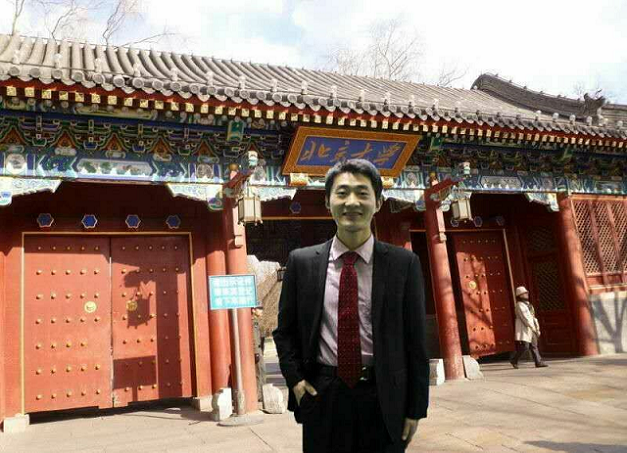
\includegraphics{shuwenhe.png}}
%写好一本书:工匠精神!用心打造!夜深写于北京大学图书馆。作者亲自一线带课,所带学生多人保送或考入清华北大,根据多年清华附中、101中学、人大附中、北大附中、十一学校,考试真题分析经验所得。用此书考上心目中名校学生无数!何书文北京大学硕士,资深数学名师、信息学竞赛算法名师,所带学生多名考入人大附中早培、清华附中优才、101 实验班、北大附中实验班等名校。全国中学数学联赛、全国中学数学竞赛的辅导老师,全国NOI、CSP信息学竞赛辅导名师。何书文老师在北京大学学习期间立志从事教育事业,帮学生授业解惑。何书文老师小学期间学习奥数,并多次获奖,为以后的学习与研究打下良好基础。何书文 老师在中学阶段数学、物理均获奖。何书文老师在小学中学期间一直为数学课代表,中小学大学期间担任班长,何书文老师在北京大学被选为科技一苑苑长,组织北大同学积极参与校各项活动,积极参与校学生会工作,何书文老师被北京大学评为优秀入党积极分子.何书文老师经常参加北京大学数学课题的研讨班。何书文 老师是北京大学数学系暑期学校全国选出40 名优秀中青年数学人才之一,参加伦敦国王学院、美国杜克大学、美国纽约大学、加拿大多伦多大学教授组成的学术研讨班,研究PDE(偏微分方程),量子力学方面的数学课题的研究工作,并获得优异成绩结业。何书文老师作为项目经理用数学建模方法给大型企业开发软件,用数学方法规划提高企业产能协作效率。何书文 老师致力于数学方面的教学与研究工作,所带多名孩子已经被点优才进入清华附中创新班,101 实验班,人大附中早培班,是家长值得信赖的老师。考上学生继续跟随何书文老师学习全国数学联赛,全国数学竞赛系列课程,同时学习NOI、IOI、ACM算法编程竞赛。
%%%%%%%%%%%%%%%%%%%%%%%%%%%%%%%%%%%%%%%%%%%%%%%%%%%%%%%%%%%%%%%%%%%%%%%%%%%%%%%%%%%%%%%%%%%%%%%%%%%%%%%%%%

%%%%%%%%%%%%%%%%%%%%%%%%%%%%%%%%%%%%%%%%%%%%%%%%%%%%%%%%%%%%%%%%%%%%%%%%%%%%%%%%%%%%%%%%%%%%%%%%%%%%%%%%%%
\title{English}
\maketitle
\tableofcontents % 显示目录
\newpage
\pagestyle{fancy}
%%%%%%%%%%%%%%%%%%%%%%%%%%%%%%%%%%%%%%%%%%%%%%%%%%%%%%%%%%%%%%%%%%%%%%%%%%%%%%%%%%%%%%%%%%%%%%%%%%%%%%%%%%

%\lhead{
\includegraphics{shuwenedu.png}}
%\rhead{科技特长生升学规划 何校长 电话微信15010729356}
%\lfoot{
\includegraphics{pku.png}算法第一人北大何书文}
%\rfoot{改变您家孩子命运的老师}
%%%%%%%%%%%%%%%%%%%%%%%%%%%%%%%%%%%%%%%%%%%%%%%%%%%%%%%%%%%%%%%%%%%%%%%%%%%%%%%%%%%%%%%%%%%%%%%%%%%%%%%%%%

%%%%%%%%%%%%%%%%%%%%%%%%%%%%%%%%%%%%%%%%%%%%%%%%%%%%%%%%%%%%%%%%%%%%%%%%%%%%%%%%%%%%%%%%%%%%%%%%%%%%%%%%%%
\begin{center}
\chapter{pronunciation}
\section{latex}
\begin{tabularx}{\textwidth}{|c|X|}
\hline
\textbf{英语音标} & \textbf{LaTeX音标} \\
\hline
\textipa{I} & \verb|\textipa{I}| \\
e & \verb|\textipa{e}| \\
\textipa{\textepsilon} & \verb|\textipa{\textepsilon}| \\
\textipa{A}& \verb|\textipa{A}| \\
\textipa{o} & \verb|\textipa{o}| \\
\textipa{U} & \verb|\textipa{U}| \\
u & \verb|\textipa{u}| \\
ə & \verb|\textipa{@}| \\
\textipa{g} & \verb|\textipa{g}| \\
\textipa{T} & \verb|\textipa{T}| \\
ð & \verb|\textipa{D}| \\
\textipa{S} & \verb|\textipa{S}| \\
\textipa{Z} & \verb|\textipa{Z}| \\
ŋ & \verb|\textipa{N}| \\
\textturnscripta & \verb|\textipa{\textturnscripta}|\\
\textipa{\textopeno} & \verb|\textipa{\textopeno}|\\
\textprimstress & \verb|\textprimstress|\\
\textipa{\textsecstress} & \verb|\textipa{\textsecstress}|\\
\textipa{\textlengthmark} & \verb|\textlengthmark|\\
\hline
\end{tabularx}
\end{center}
\section{26个字母}
\begin{tabular}{|c|c|c|c|c|c|c|c|c|c|c|c|c|c|c|c|c|c|c|c|c|c|c|c|c|c|c|}
  \hline
  A & B & C & D & E & F & G & H & I & J & K & L & M & N & O & P & Q & R & S & T & U & V & W & X & Y&Z\\
  a & b & c & d & e & f & g & h & i & j & k & l & m & n & o & p & q & r & s & t & u & v & w & x & y&z\\
  \hline
\end{tabular}
\section{48个国际音标}
\subsection{前元音\textipa{I}}
\begin{tabular}{|c|c|c|}
\hline
词汇 & 音标 & 译意 \\
\hline
kit & /k\textipa{I}t/ & n. 成套工具 \\
bid & /b\textipa{I}d/ & n. 投标 \\
hymn & /h\textipa{I}m/ & n. 圣歌 \\
minute & /\textprimstress m\textipa{I}n\textipa{I}t/ & n. 分钟;会议记录 \\
\hline
\end{tabular}
\subsection{前元音\textipa{I}\textlengthmark}
\begin{tabular}{|c|c|c|}
\hline
词汇 & 音标 & 译意 \\
\hline
hit & /h\textipa{I}t/ & n. 打击 \\
heat & /h\textipa{I}\textipa{\textlengthmark}t/ & n. 热能 \\
\hline
sick & /s\textipa{I}k/ & n. 病人  \\
seek & /s\textipa{I}\textipa{\textlengthmark}k/ & v. 寻找 \\
\hline
\end{tabular}

\chapter{vocabulary}
\section{a}
\begin{tabular}{|c|c|c|c|c|}
\hline
英文 & 音标 & 中文 & 词根词缀 & 词组\\
\hline
adjacency & /ə\textprimstress d\textipa{Z}e\textipa{I}sənsi/ & n. 邻接 & & adjacency list 邻接表 adjacency matrix 邻接矩阵 \\
assign & /əˈsaɪn/ & v. 分配 & & \\
algorithm & /\textprimstress æl\textipa{g}ər\textipa{I}ðəm/ & n. 算法 & & \\
\hline
\end{tabular}

\section{b}
\begin{tabular}{|c|c|c|c|c|}
\hline
英文 & 音标 & 中文 & 词根词缀 & 词组\\
\hline
barn & /bɑːn/ & n. 谷仓 & & born出生\\
\hline
bipartite & /ba\textipa{I}\textprimstress p\textipa{A}\textlengthmark ta\textipa{I}t/ & adj. 二分的 & & bipartite graph 二分图\\
\hline
\end{tabular}

\section{c}
\begin{tabular}{|c|c|c|c|c|}
\hline
英文 & 音标 & 中文 & 词根词缀 & 词组\\
\hline
contest & /ˈkɒntest/ & n. 比赛 & &\\
competition& /ˌkɒmpəˈtɪʃ(ə)n/ & n. 竞赛 & &\\
candy & /\textprimstress kændi/ & n. 糖果 & &\\
constant & /ˈkɒnstənt/ & n. 常数 & & constant value 常数值\\
complement & /ˈkɒmplɪment/ & n. 补集 & &\\
\hline
\end{tabular}

\section{d}
\begin{tabular}{|c|c|c|c|c|}
\hline
英文 & 音标 & 中文 & 词根词缀 & 词组\\
\hline
dijkstra & /ˈdaɪkstrə/ & n. 迪杰斯特拉 & & \\
directive & /dəˈrektɪv/ & n. 指令 & & preprocessor directive预处理器指令\\
declared\\
dynamic & /daɪˈnæmɪk/ & & &  dynamic prgramming动态规划\\
\hline
\end{tabular}

\section{e}
\begin{tabular}{|c|c|c|c|}
\hline
词汇 & 音标 & 译意 & 词根词缀\\
\hline
element & /\textprimstress el\textipa{I}mənt/ & n. 元素& \\
logical expression\\
\hline
\end{tabular}

\section{f}
\begin{tabular}{|c|c|c|c|c|}
\hline
英文 & 音标 & 中文 & 词根词缀 & 词组\\
\hline
factorial & /fækˈtɔːriəl/ & n. [数] 阶乘 & &\\
\hline
\end{tabular}
\section{g}
\begin{tabular}{|c|c|c|c|}
\hline
词汇 & 音标 & 译意 & 词根词缀\\
\hline
greedy & /\textprimstress\textipa{g}ri\textlengthmark di/ & adj. 贪心的& \\
graph & /ɡrɑːf/ & adj. 贪心的& \\
\hline
\end{tabular}
\section{h}
\section{i}
\begin{tabular}{|c|c|c|c|c|}
\hline
英文 & 音标 & 中文 & 词根词缀 & 词组\\
infinity  & /ɪnˈfɪnəti/ & n. 无穷 & &\\
increment & /\textprimstress\textipa{I}ŋkrəmənt/ & 自增 & in- 入 , 向内 + -cre- 生长 + -ment 名词词尾 &\\
implementation & /\textipa{\textsecstress}\textipa{I}mpl\textipa{I}men\textipa{\textprimstress}te\textipa{I}\textipa{S}(ə)n/ & n. 实现& &\\
International & & & International Phonetic Alphabet国际音标&\\
\hline
\end{tabular}

\section{j}
\section{k}
\section{l}
logical expression

\section{m}
\begin{tabular}{|c|c|c|c|c|}
\hline
英文 & 音标 & 中文 & 词根词缀 & 词组\\
\hline
mathematics & /\textipa{\textsecstress}mæ\textipa{T}ə\textprimstress mæt\textipa{I}ks/ & n. 算法 & \\
modify & /\textprimstress m\textturnscripta d\textipa{I}fa\textipa{I}/ & v. 修改 & -mod- 量器 + -i- + -fy 动词词尾\\
macro & /ˈmækrəʊ/ & n. (计算机)宏 & &  defines a macro定义一个宏\\
memorization & /ˌmeməˈrɪzeɪʃən/ & n. (计算机)宏 & &  memorization search 记忆搜索\\
\hline
\end{tabular}

\section{n}
\begin{tabular}{|c|c|c|c|c|}
\hline
英文 & 音标 & 中文 & 词根词缀 & 词组\\
\hline
nuked & /nju\textlengthmark kt/ & 核武器 & & bool nuked[maxN]; // 标记节点是否已被处理\\
\hline
\end{tabular}

\section{o}
\begin{tabular}{|c|c|c|c|}
\hline
词汇 & 音标 & 译意 & 词根词缀\\
\hline
origin & /\textprimstress\textipa{\textopeno}\textipa{\textlengthmark}r\textipa{I}d\textipa{Z}\textipa{I}n/ & n. 起源& \\
original & /ə\textprimstress r\textipa{I}d\textipa{Z}ən(ə)l/ & adj. 起初的& \\
operator & /ˈɒpəreɪtə(r)/ & n.运算符 & \\
overload & /ˌəʊvəˈləʊd/ & v. 重载 & \\
operator & /ˈɒpəreɪtə(r)/ & n. 运算符 & \\
\hline
\end{tabular}

\section{p}
\begin{tabular}{|c|c|c|c|c|}
\hline
英文 & 音标 & 中文 & 词根词缀 & 词组\\
\hline
priority & /praɪˈɔːrəti/ & v. 优先 &  & priority queue 优先队列\\
prune & /pru\textlengthmark n/ & v. 修剪 & &\\
prime & /praɪm/ & n. 素数 & &\\
proxy & /ˈprɒksi/ & n. 代理 & &\\
preprocessor & /ˌpriːˈprəʊsesə/ & n. 预处理器 & & preprocessor directive预处理器指令\\
positive & /ˈpɒzətɪv/ & n. 正数 & & positive value 正值\\
provide& /prəˈvaɪd/ & v. 提供 & & provided by 由......提供\\
permission&  & v. 提供 & & permission denied 权限拒绝\\
power& /ˈpaʊər/ & v. 提供 & & permission denied 权限拒绝\\
pair& /peə(r)/ & v. 提供 & & permission denied 权限拒绝\\
\hline
\end{tabular}

\section{q}
\section{r}
\begin{tabular}{|c|c|c|c|}
\hline
词汇 & 音标 & 译意 & 词根词缀\\
\hline
reference & /\textprimstress refrəns/ & 引用 & re- 回 + -fer- 拿取 + -ence 名词词尾\\
represent & /ˌreprɪˈzent/ & v.表示 &\\
recursive & /r\textipa{I}\textprimstress k\textipa{Z}\textipa{\textlengthmark}s\textipa{I}v/ & adj. [数] 递归的 &recur, 复发,再次发生,引申词义循环的\\
\hline
\end{tabular}

\section{s}
scope
\section{t}
\begin{tabular}{|c|c|c|c|}
\hline
词汇 & 音标 & 译意 & 词根词缀\\
\hline
temp & /temp/ & 临时变量 & \\
\hline
\end{tabular}
\section{u}
\begin{tabular}{|c|c|c|c|c|}
\hline
英文 & 音标 & 中文 & 词根词缀 & 词组\\
\hline
unreachable & /ʌn'ri:tʃəbl/ & adj. 不能达到的 & &unreachable distance遥不可及的距离\\
\hline
\end{tabular}
\section{v}
\begin{tabular}{|c|c|c|c|c|}
\hline
词汇 & 音标 & 译意 & 词根词缀 & 复数\\
\hline
vector & /\textprimstress vektər/ & 向量 & &\\
vertex & /ˈvɜːteks/ & n. 顶点 & & vertices\\
valid & /ˈvælɪd/ & adj.合法的 & & \\
\hline
\end{tabular}
\section{w}
\section{x}
\section{y}
\section{z}

\section{Category}
\subsection{Month}
\begin{tabular}{|c|c|c|c|}
\hline
英文 & 音标 & 中文 & 词根词缀\\
\hline
month & /mʌnθ/ & n. 月 & \\
\hline
Jan(January) & /ˈdʒænjuəri/ & n. 一月 & \\
Feb(February) & /ˈfebruəri/ & n. 二月 & \\
Dec(December) & /dɪˈsembə(r)/ & n. 十二月 & \\
\hline
\end{tabular}

\subsection{Level}
\begin{tabular}{|c|c|c|c|}
\hline
英文 & 音标 & 中文 & 词根词缀\\
\hline
Platinum & /ˈplætɪnəm/ & n. 铂金 & \\
Gold & /ɡəʊld/ & n. 金 & \\
Silver & /ˈsɪlvə(r)/ & n. 银 & \\
\hline
\end{tabular}

\chapter{grammar}
\section{主语}
Chuck is a businessman.
\section{谓语}
Chuck is a businessman.
\section{宾语}
Chuck is a businessman.
\section{定语从句}
\subsection{who}
\subsubsection{}
He was an old man who fished alone in a skiff in the Gulf Stream. 
\subsubsection{}
Chuck is a businessman who is always so busy that he has little time for his friends. \\
主语:Chuck\\
谓语:is\\
宾语:a businessman\\
定语从句:who is always so busy从句是用来修饰名词或代词的从句,修饰名词"businessman",限定了Chuck的身份和特征,描述了他总是非常忙碌。\\
补语:who is always so busy that he has little time for his friends\\
补充说明:\\
- "is" 是谓语动词,表示状态或身份。\\
- "a businessman" 是宾语,描述了Chuck的身份。\\
- "who is always so busy that he has little time for his friends" 是补语,进一步描述了Chuck的状态。这个从句中包含了一个关系代词"who"和一个从属连词"that",连接了两个子句。"who"引导一个定语从句,修饰先行词"businessman",并描述了他的状态。"that"引导一个结果状语从句,说明他非常忙碌,以至于没有时间和朋友们相处。
\section{状语从句}
Chuck is a businessman who is always so busy that he has little time for his friends. \\
"that"引导一个结果状语从句
\section{补语}
Chuck is a businessman who is always so busy that he has little time for his friends. \\
补语:是用来补充、说明或描述主语或宾语的成分。在这个句子中,补语是"who is always so busy that he has little time for his friends"。它进一步描述了主语Chuck的状态,即他非常忙碌,以至于没有时间和朋友们相处。

\chapter{sentence}
\section{d}
error: ‘z’ was not declared in this scope.\\
错误:“z”未在此范围内声明.

\section{New Concept新概念}
\subsection{第一册}
\subsection{第二册}
\subsection{第三册}
\subsection{第四册}
\section{The Old Man and the Sea}
\subsection{01}
He was an old man who fished alone in a skiff in the Gulf
Stream and he had gone eighty-four days now without taking
a fish. In the first forty days a boy had been with him.\\
他是个独自在湾流中一条小船上钓鱼的老人,至今已去了八十四天,
一条鱼也没有逮住。前四十天里,有个男孩子跟他在一起。\\
But after forty days without a fish the boy's parents had told
him that the old man was now definitely and finally salao,
which is the worst form of unlucky, and the boy had gone at
their orders in another boat which caught three good fish the
first week. It made the boy sad to see the old man come in
each day with his skiff empty and he always went down to
help him carry either the coiled lines or the gaff and harpoon
and the sail that was furled around the mast.\\
可是,过了四十天还没捉到一条鱼,孩子的父母对他说,老人如今准
是十足地“倒了血霉”,这就是说,倒霉到了极点,于是孩子听从了他
们的吩咐,上了另外一条船,头一个礼拜就捕到了三条好鱼。孩子看
见老人每天回来时船总是空的,感到很难受,他总是走下岸去,帮老人
拿卷起的钓索,或者鱼钩和鱼叉,还有绕在桅杆上的帆。\\
The sail was patched with flour sacks and, furled, it looked
like the flag of permanent defeat. The old man was thin and
gaunt with deep wrinkles in the back of his neck.\\
帆上用面粉袋片打了些补丁,收拢后看来象是一面标志着永远失败的
旗子。老人消瘦而憔悴,脖颈上有些很深的皱纹。\\
The brown blotches of the benevolent skin cancer the sun
brings from its reflection on the tropic sea were on his
cheeks. The blotches ran well down the sides of his face and
his hands had the deep-creased scars from handling heavy
fish on the cords.\\
腮帮上有些褐斑,那是太阳在热带海面上反射的光线所引起的良性皮肤改变。褐斑从他脸的两侧一直蔓延下去,他的双手常用绳索拉鱼,留下了刻得很深的伤疤。
\subsection{02}

\subsection{03}
\subsection{04}
\subsection{05}
\subsection{06}
\subsection{07}
\subsection{08}
\subsection{09}
\subsection{10}
\subsection{11}
\subsection{12}
\subsection{13}
\subsection{14}
\subsection{15}
\subsection{16}
\subsection{17}
\subsection{18}
\subsection{19}
\subsection{20}
\subsection{21}
\subsection{22}
\subsection{23}
\subsection{24}
\subsection{25}
\subsection{26}
\subsection{27}
\subsection{28}
\subsection{29}
\subsection{30}
\subsection{31}
\subsection{32}
\subsection{33}
\subsection{34}
\subsection{35}
\subsection{36}
\subsection{37}
\subsection{38}
\subsection{39}
\subsection{40}
\subsection{41}
\subsection{42}
\subsection{43}
\subsection{44}
\subsection{45}
\subsection{46}
\subsection{47}
\subsection{48}
\subsection{49}
\subsection{50}
\subsection{51}

\clearpage
\end{document}
